\section{The Poisson Distribution}
\subsection{The Poisson Distribution}

{Poisson Distribution} We say that a \emph{discrete} random variable $X$ has a Poisson distribution if its probability function is given by:
 \begin{align}
  \label{eq:2.10.7}
  f(n)=\dfrac{\lam^{n}e^{-\lam}}{n!}, \; n=0,1,2,...
 \end{align}

In this case, $\mu_{X}=\s^{2}=\lam.$

\begin{quote}
 In probability theory and statistics, the Poisson distribution is a discrete probability distribution that expresses, from a mean frequency of occurrence, the probability that a given number of events occurs during a certain period of time. It specializes in the probability of rare events or events with very small probabilities.
\end{quote}

\href{https://en.wikipedia.org/wiki/Poisson_distribution}{Wikipedia: Poisson Distribution}

\begin{ejemplo}
  \label{exmp:2.10.5}
  The number of people arriving per day at an emergency room follows a Poisson distribution with mean 5. Find the probability that at most three arrive per day and the probability that at least 8 people arrive per day.
\end{ejemplo}

\begin{solucion}
	Using the Poisson distribution with $\lambda = 5$:

	\begin{enumerate}
		\item $P(X \leq 3) = \sum_{n=0}^{3} \frac{5^n e^{-5}}{n!}$
		\begin{align}
			&= \frac{5^0 e^{-5}}{0!} + \frac{5^1 e^{-5}}{1!} + \frac{5^2 e^{-5}}{2!} + \frac{5^3 e^{-5}}{3!} \\
			&= e^{-5}(1 + 5 + 12.5 + 20.833) \\
			&= e^{-5} \cdot 39.333 \approx 0.265
		\end{align}

		\item $P(X \geq 8) = 1 - P(X \leq 7)$
		\begin{align}
			&= 1 - \sum_{n=0}^{7} \frac{5^n e^{-5}}{n!} \\
			&\approx 1 - 0.867 = 0.133
		\end{align}
	\end{enumerate}
\end{solucion}

\lstinputlisting[language=Python]{../code/distribuciones-especiales/distPoisson.py}

 \begin{figure}
 \centering
 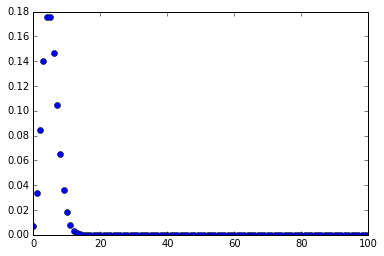
\includegraphics[height=7cm,keepaspectratio=true]{./pe/distPoisson0.png}
 % distPoisson0.png: 0x0 pixel, 300dpi, 0.00x0.00 cm, bb=
 \caption{Poisson Distribution}
\end{figure}

\begin{figure}
 \centering
 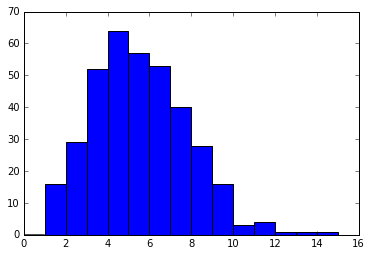
\includegraphics[height=7cm,keepaspectratio=true]{./pe/distPoisson1.png}
 % distPoisson1.png: 0x0 pixel, 300dpi, 0.00x0.00 cm, bb=
 \caption{Histogram of emergency room patients over a year with mean $\lam=5$}
 \label{fig:2.10.6}
\end{figure}

\subsection{Relationship Between the Binomial and Poisson Distributions}

If in the binomial probability function $N$ is very large while $p \approx 0,$ this models a \emph{rare event}. In practice, this means $N>>50, Np<<5.$

In this case, the binomial distribution with parameters $N,p$ approaches a Poisson distribution with parameter $\lam = Np.$

\lstinputlisting[language=Python]{../code/distribuciones-especiales/relBinomPoisson.py}

 \begin{figure}
 \centering
 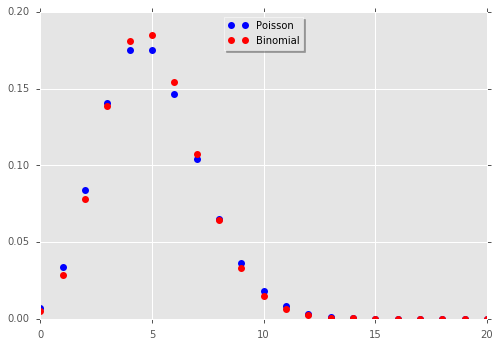
\includegraphics[height=7cm]{./pe/binVsPoi.png}
 % binVsPoi.png: 0x0 pixel, 300dpi, 0.00x0.00 cm, bb=
 \caption{Comparison between Binomial and Poisson distributions for rare events.}
\end{figure}

\subsection{Normal Approximation to Discrete Distributions}
\subsubsection{Normal Distribution}

One of the most important continuous probability distributions is the \emph{normal distribution}, also called the \emph{Gaussian distribution}, which is defined by the density function
 \begin{align}
  \label{eq:2.10.4}
  f_{a,b}(x)=\dfrac{1}{\sqrt{2\pi}}e^{-\frac{1}{2}\frac{(x-a)^{2}}{b^{2}}}
 \end{align}
where $a,b$ are specific parameters for each random variable $X.$

{Properties of the normal distribution}
If the random variable $X$ has the density function given by \eqref{eq:2.10.4}, with parameters $a,b$, then
 \begin{align}
  a = \mu_{X}\\
  b = \s_{X}
 \end{align}

If a normal random variable $X$ has density function
  \begin{align}
  \label{eq:2.10.4a}
  f(x)=\dfrac{1}{\sqrt{2\pi}}e^{-\frac{1}{2}\frac{(x-\mu)^{2}}{\s^{2}}},
  \end{align}
  we write $X\sim N(\mu, \s^{2}).$

{Standardized random variable}
 \begin{align}
  \label{eq:2.10.5}
  Z = \dfrac{X-\mu}{\s}\\
  \mu_{Z}=0 \\
  \s_{Z}=1
 \end{align}

{Standard form}
 \begin{align}
  \label{eq:2.10.6}
  f(z)=\dfrac{1}{\sqrt{2\pi}}e^{-\frac{1}{2}z^{2}}
 \end{align}

In this case, we say that $Z$ is \emph{normally distributed.}

\lstinputlisting[language=Python]{../code/distribuciones-especiales/distribucionNormal.py}

 \begin{figure}
 \centering
 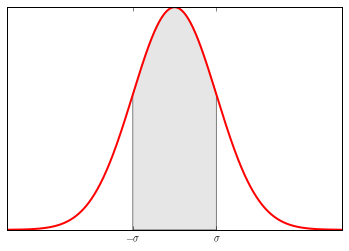
\includegraphics[height=5cm,keepaspectratio=true]{./pe/norm1.png}
 % norm1.png: 0x0 pixel, 300dpi, 0.00x0.00 cm, bb=
 \label{fig:2.10.2}
\end{figure}
\begin{verbatim}
 #(0.682689492137086, 7.579375928402476e-15)
\end{verbatim}

 \begin{figure}
 \centering
 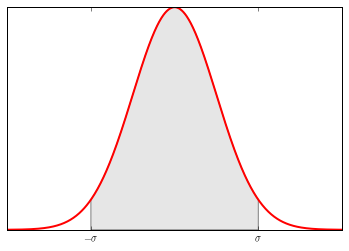
\includegraphics[height=5cm,keepaspectratio=true]{./pe/norm2.png}
 % norm2.png: 0x0 pixel, 300dpi, 0.00x0.00 cm, bb=
 \label{fig:2.10.3}
\end{figure}
\begin{verbatim}
 #(0.9544997361036417, 1.8403548653972355e-11)
\end{verbatim}

 \begin{figure}
 \centering
 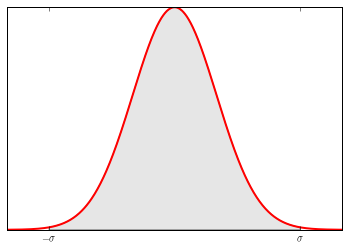
\includegraphics[height=5cm,keepaspectratio=true]{./pe/norm3.png}
 % norm3.png: 0x0 pixel, 300dpi, 0.00x0.00 cm, bb=
 \label{fig:2.10.4}
\end{figure}
\begin{verbatim}
 #(0.9973002039367399, 1.1072256503105314e-14)
\end{verbatim}

 \begin{figure}
 \centering
 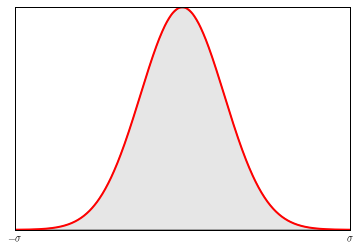
\includegraphics[height=5cm,keepaspectratio=true]{./pe/norm4.png}
 % norm4.png: 0x0 pixel, 300dpi, bb=0x0
 \label{fig:2.10.5}
\end{figure}
\begin{verbatim}
 #(0.9999366575163339, 4.838904125482879e-12)
\end{verbatim}

\lstinputlisting[language=Python]{../code/distribuciones-especiales/normalCDF.py}
\begin{center}
 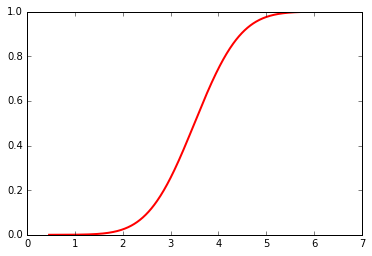
\includegraphics[height=5cm,keepaspectratio=true]{./pe/normCDF.png}
 % normCDF.png: 0x0 pixel, 300dpi, 0.00x0.00 cm, bb=
\end{center}

\subsubsection{Relationship between the binomial and normal distributions}

If $N\sim \infty, p,q>>0,$ and $X$ is a binomial random variable with parameters $N,p$, then
 \begin{align}
  \dfrac{X-Np}{\sqrt{Npq}} \sim N(0,1).
 \end{align}

\begin{ejemplo}
  \label{exmp:2.10.4}
  Consider the experiment of tossing a coin 16 times. Repeat this experiment 1,000,000 times. Verify that it can be modeled by a random variable with distribution $N(\mu=8,\sigma^{2}=4).$
\end{ejemplo}

\lstinputlisting[language=Python]{../code/distribuciones-especiales/relBinomNormal.py}
\begin{center}
 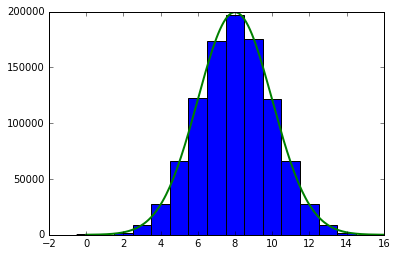
\includegraphics[height=5cm]{./pe/relBinNorm.png}
 % relBinNorm.png: 0x0 pixel, 300dpi, bb=0x0
\end{center}

\subsubsection{Solved Problems}

{Percentile}
We say that $x=P_{q}$ is the percentile $q, \; 0\leq q \leq 100$ of the distribution $F(x)$ if $F(P_{q})=q\%.$ When $q$ is a realizable value of $F(x),$ we can \emph{solve for}
 \begin{align}
  P_{q}=F^{-1}\left( \dfrac{q}{100} \right).
 \end{align}
Such a function is called an \emph{inverse distribution.}

{Quartiles}
Similar concepts are defined in the literature. For example, the first \emph{quartile} corresponds to percentile $25;$ the second quartile to percentile $50;$ and so on.

{Combinations}
\begin{ejemplo}
  \label{exmp:2.10.7}
  Find
  \begin{enumerate}
   \item $5!$
   \item $\comb{8}{3}$
  \end{enumerate}
  using \texttt{Python.}
\end{ejemplo}

\lstinputlisting[language=Python]{../code/distribuciones-especiales/combinaciones.py}

{Binomial Distribution}
\begin{ejemplo}
  \label{exmp:2.10.8}
  Suppose that $15\%$ of the population is left-handed. Find the probability that in a group of 50 individuals there are:
  \begin{enumerate}
   \item at most 10 left-handed people;
   \item at least 5 left-handed people;
   \item between 3 and 6 left-handed people;
   \item exactly 5 left-handed people.
  \end{enumerate}
\end{ejemplo}

\lstinputlisting[language=Python]{../code/distribuciones-especiales/solvedBinom.py}

{Normal Distribution}
\begin{ejemplo}
  \label{exmp:2.10.9}
  On a final mathematics exam, the mean was 72 and the standard deviation was 15. Determine the standardized scores of students who obtained:
  \begin{enumerate}
   \item $60$;
   \item $93$;
   \item $72$.
  \end{enumerate}
\end{ejemplo}

\begin{ejemplo}
   \label{exmp:2.10.10}
   Using the data from Example \ref{exmp:2.10.9}, find the grades corresponding to the following standardized scores:
  \begin{enumerate}
   \item $-1$;
   \item $1.6$.
  \end{enumerate}
\end{ejemplo}

\begin{ejemplo}
  \label{exmp:2.10.11}
  Suppose that the number of games in which major league baseball players participate during their careers is normally distributed with mean 1500 games and standard deviation 350 games. Use \texttt{Python} to answer:
  \begin{enumerate}
   \item What percentage participate in fewer than 750 games?
   \item What percentage participate in more than 2000 games?
   \item Find the 90th \emph{percentile} of the number of games in which they participate during their careers.
  \end{enumerate}
\end{ejemplo}

\lstinputlisting[language=Python]{../code/distribuciones-especiales/solvedNorm.py}

{Rare Events}
\begin{ejemplo}
\label{exmp:2.10.12}
If the probability that an individual has an adverse reaction to an injection of a given serum is $0.001,$ determine the probability that out of 2000 individuals:
 \begin{enumerate}
  \item exactly 3;
  \item more than 2
 \end{enumerate}
suffer an adverse reaction.
\end{ejemplo}

\lstinputlisting[language=Python]{../code/distribuciones-especiales/eventosRaros.py}
